\documentclass[tikz,border=5pt]{standalone}
\begin{document}
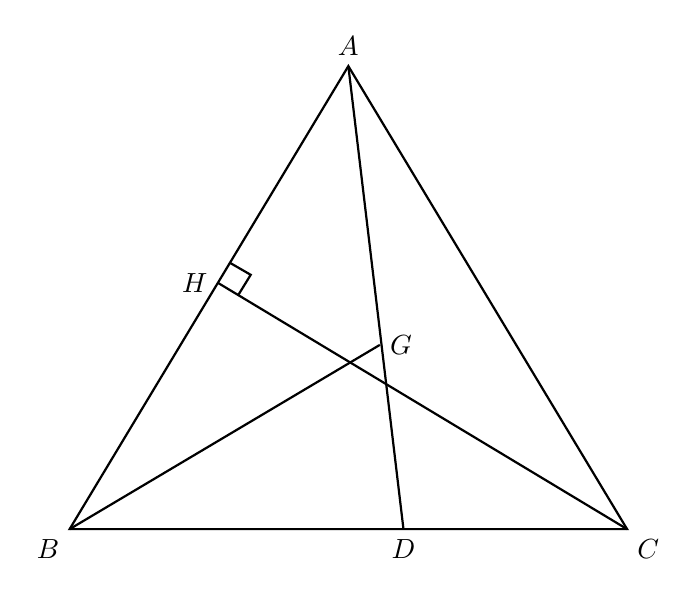
\begin{tikzpicture}[line width=0.8pt]
  % 坐标定义
  \coordinate (A) at (4.94,-1.34);
  \coordinate (B) at (1.40,-7.22);
  \coordinate (C) at (8.48,-7.22);
  \coordinate (D) at (5.64,-7.22);
  \coordinate (G) at (5.34,-4.88);
  \coordinate (H) at (3.28,-4.09);

  % 原图元：三角形 ABC、线段 AD、线段 BG
  \draw (A) -- (B) -- (C) -- cycle;
  \draw (A) -- (D);
  \draw (B) -- (G);

  % 新增：从 C 到 AB 的垂线 CH
  \draw (C) -- (H);

  % 直角标记
  \draw (3.44,-3.84) -- (3.70,-3.99) -- (3.54,-4.25);

  % 标签
  \node[above] at (A) {$A$};
  \node[below left] at (B) {$B$};
  \node[below right] at (C) {$C$};
  \node[below] at (D) {$D$};
  \node[right] at (G) {$G$};
  \node[left] at (H) {$H$};
\end{tikzpicture}
\end{document}
